\documentclass{article}
\usepackage[utf8]{inputenc}

\title{Análisis Exploratorio de Datos \\ Trabajo Práctico 1 - Organización de Datos}
\author{Nombre de grupo}
\date{Poner fecha}

\usepackage{natbib}
\usepackage{graphicx}
\newcommand\tab[1][1cm]{\hspace*{#1}}
\usepackage{placeins}

\begin{document}
\begin{figure}
    \centering
    \makebox[\textwidth]{
\includegraphics[width=250pt]{logofiuba.jpg}}
\end{figure}

\maketitle

\FloatBarrier
\begin{center}
        \begin{tabular}{ |c|c|c| }
          \hline
          Nombre & Padrón & Mail \\
          \hline\hline
          Álvarez, Federico & 99266 & fede.alvarez1997@gmail.com \\
          \hline
          La Torre, Gabriel & 87796 & latorregab@gmail.com \\
          \hline
          Medrano, Lucas Nicolás & 99247 & lucasmedrano97@gmail.com \\
          \hline
          Piro Martino, Ariel & 99469 & ariel.piro@hotmail.com \\
          \hline
        \end{tabular}
\end{center}
\FloatBarrier

\newpage

\tableofcontents
\newpage
\section{Introduction}
	\tab En el trabajo se hace un análisis exploratorio de un set de datos provistos por la empresa Jampp. En el mismo se encuentra información de subastas, instalaciones, clicks, entre otros.\\
	\tab Primero se hará una visión general de los archivos (installs.csv, clicks.csv, auctions.csv, events.csv) para entender la distribución y la cantidad de datos, el significado de las columnas, reconocer las columnas que no aportan información (por ejemplo, las que tienen todos sus valores nulos), reconocer el tipo de datos en cada columna, seguido de un análisis mas profundo para obtener mas información de los datos. Luego se hará un análisis global, buscando información relativa a los archivos en conjunto, permitiendo obtener otro tipo de información.

\section{Análisis individual de archivos}
\subsection{Subastas}
	\subsubsection{Análisis general}
	 \tab El archivo 'auctions.csv' contiene información acerca de subastas.
	Hay dos columnas que no nos aportan información significante. 'auction\_type\_id' tiene todos sus valores 		nulos, por lo que no fue tomada en cuenta para el análisis. 'country' informa un solo valor posible, que se supone que debe ser Argentina.
	\tab La columna platforms tiene dos valores posibles (1 y 2) que se supone son Android e iOS. Va a ser importante para el análisis que hagamos más adelante. De ahora en más, platform y sistema operativo serán sinónimos en este informe.
	\tab Por último, 'source' nos da información acerca del exchange de donde surge la subasta.
	\tab Además vemos que ningún valor de este archivo, excluyendo la columna 'auction\_type\_id', es nulo, por lo que no es necesario tomar ninguna decisión respecto a eso.
	
	\subsubsection{Subastas por día de Marzo}
	\tab Como primer acercamiento a este set de datos, es interesante ver cómo se distribuye la cantidad de subastas en los días que incluye el archivo (05/03/19 al 13/03/19). El gráfico \ref{subastasmarzo} representa dicha distribución. En él se pueden observar varias cosas:
	\begin{itemize}
		\item La cantidad de subastas parece, en general, aumentar con el paso de los dias.
		\item El valor del último día es mas del doble del valor del primer día.
		\item El mayor aumento se da del sexto al septimo día.
		\item La cantidad de subastas varía entre unos valores extremos, aproximados, de un millón y 3 millones.
	\end{itemize}
	\FloatBarrier
		\begin{figure}
			\centering
			   	\makebox[\textwidth]{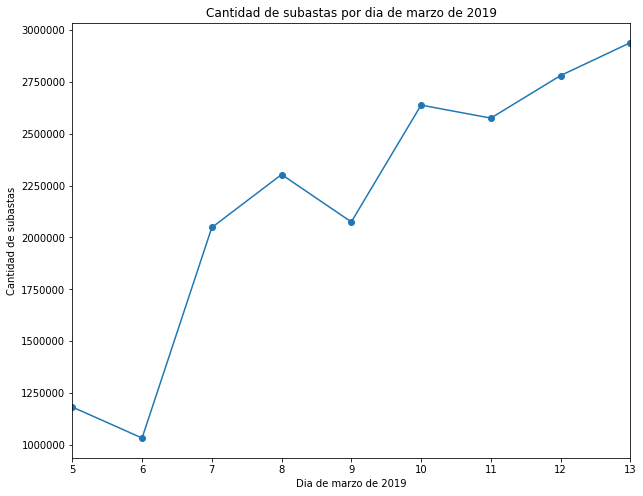
\includegraphics[width=300pt]{images/auctions/subastaspordia.png}}
		   		\caption{Cantidad de subastas por día de Marzo}
			   	\label{subastasmarzo}
		\end{figure}
	\FloatBarrier
			
	\subsubsection{Subastas por día de Marzo por sistema operativo}
	\tab Otro punto interesante es dividir el problema. Obtener la distribución de subastas en los días con datos disponibles para cada plataforma (Android e iOS). En la imagen \ref{subastasmarzoSO} se pueden observar las cantidades. Observese que llamamos '1' y '2' a las plataformas, ya que no sabemos cuál es Android y cuál es iOS.
	\tab Puntos interesantes a reconocer:
	
	\begin{itemize}
		\item La cantidad de subastas para la plataforma '1' es, salvo en el cuarto y el quinto día, considerablemente mayor a la cantidad para la plataforma '2'.
		\item La figura de la plataforma '2' es mucho mas "chata" que la de la plataforma '1', la cual representa mas picos y saltos.
		\item La figura de la plataforma '1' es muy parecida a la del gráfico \ref{subastasmarzo}, mientras que la de la plataforma '2' no lo es. Esto es resultado, principalmente, de lo indicado en el primer ítem. Este análisis puede llegar a ser muy útil para reconocer partes de los datos que son representativas del total.
	\end{itemize}
	\FloatBarrier
		\begin{figure}
			\centering
	   		\makebox[\textwidth]{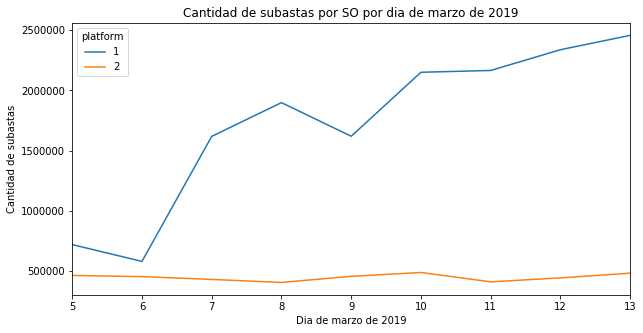
\includegraphics[width=350pt]{images/auctions/subastaspordiaSO.png}}
		   	\caption{Cantidad de subastas por día de Marzo y por sistema operativo}
		   	\label{subastasmarzoSO}
		\end{figure}
	\FloatBarrier
			
	\subsubsection{Subastas por hora del día}
	\tab Ahora vamos a analizar cómo se distribuyen las subastas a lo largo del día. Para esto hacemos un gráfico de hora del día contra cantidad de subastas (Gráfico \ref{subastashora}).\newline
	\tab Desde un análisis cualitativo se pueden observar algunos puntos:
	\begin{itemize}
		\item Parece ser que la mayor cantidad de subastas se distribuyen por la noche y la madrugada.
		\item La cantidad de subastas es poca en horas de la mañana y el mediodía. En el gráfico se puede ver un gran valle en esa parte del día.
	\end{itemize}
	
	\FloatBarrier
		\begin{figure}[ht!]
			\centering
			\makebox[\textwidth]{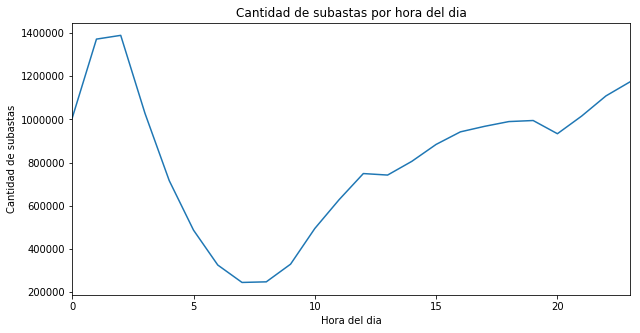
\includegraphics[width=350pt, bb=0 0 640 480]{images/auctions/subastasporhora.png}}
		   	\caption{Cantidad de subastas por hora del día}
			\label{subastashora}
		\end{figure}
	\FloatBarrier
	\subsubsection{Subastas por hora del día por sistema operativo}
	\tab Al igual que se hizo antes, podemos dividir el gráfico para ambas plataformas. Vemos que pasa algo muy parecido que lo que pasaba para la cantidad de subastas por día. El gráfico de la plataforma '1', al tener una cantidad mucho mayor de subastas, es la que predomina en el gráfico de la sección "Subastas por hora del día", y por eso sus gráficos son tan parecidos. EL gráfico de la plataforma '2' es bastante mas chato, y con cantidades de subastas mucho mas chicas.

	\FloatBarrier
		\begin{figure}
			\centering
			\makebox[\textwidth]{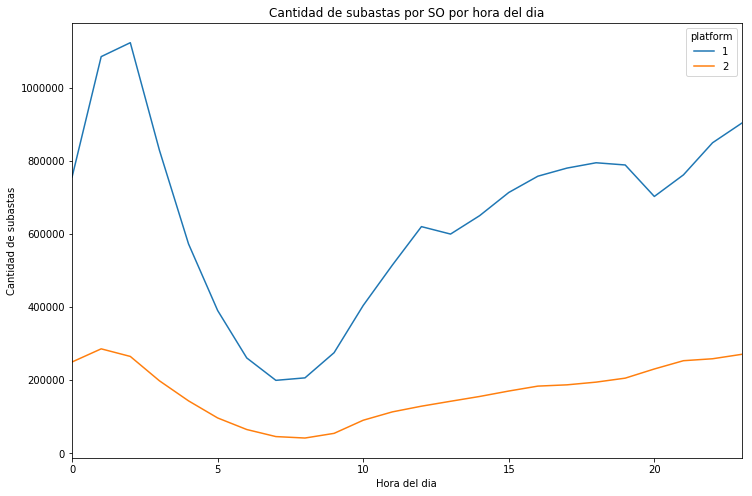
\includegraphics[width=220pt]{images/auctions/subastasporhoraS0.png}}
		   	\caption{Cantidad de subastas por hora del día por sistema operativo}
			\label{subastashoraSO}
		\end{figure}
	\FloatBarrier	
	
	\subsubsection{Subastas por sistema operativo}
	\tab Resulta interesante conocer cuál es el sistema operativo para el cual se generan más subastas. Es algo que ya se venía viendo en la forma y nivel (cantidad de subastas) de los gráficos anteriores. Sin embargo, los gráficos vistos hasta ahora no dan un conocimiento directo de la relacion de las cantidades de subastas de ambas plataformas. 
	\tab En las figuras que se ven a continuación podemos confirmar que lo que indicabamos en los gráficos anteriores era cierto. La cantidad de subastas es mucho mayor para la plataforma '1'. Además, ahora tenemos una visión mas cuantitativa de esta relación (en la imagen \ref{subastasSOporcentajes} vemos una relación porcentual, mientras que la imagen \ref{subastasSOcantidades} nos da mas idea de las cantidades).
	
	\FloatBarrier
		\begin{figure}
			\centering
			\makebox[\textwidth]{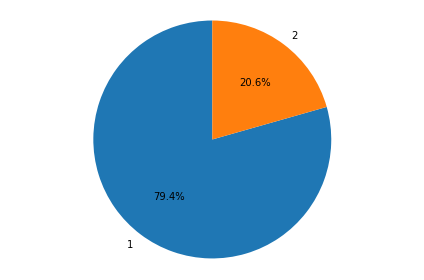
\includegraphics[width=350pt]{images/auctions/subastasporSO.png}}
		   	\caption{Porcentaje de subastas para cada plataforma}
			\label{subastasSOporcentajes}
		\end{figure}
	\FloatBarrier
	
	\FloatBarrier
		\begin{figure}
			\centering
			\makebox[\textwidth]{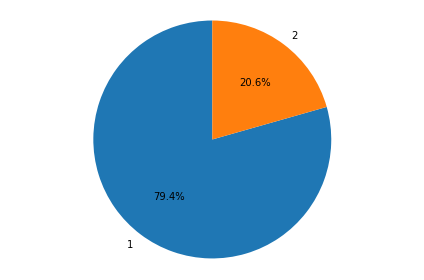
\includegraphics[width=350pt]{images/auctions/subastasporSO.png}}
		   	\caption{Porcentaje de subastas para cada plataforma}
			\label{subastasSOcantidades}
		\end{figure}
	\FloatBarrier	
	
	\subsubsection{Subastas por source}
	\tab Como indica la introducción a esta sección (vease Auctions/Análisis general), source nos indica el exchange que generó la subasta. Se puede obtener, a partir de los datos, cuáles son los exchanges principales, y cuántas subastas generan.
	\tab A tener en cuenta:
	\begin{itemize}
		\item Los que se muestran son todos los exchanges que aparecen en el archivo.
		\item Al igual que en las plataformas, los exchanges se toman por un id, y no por su nombre.
		\item Hay una clara diferencia en las cantidades.
		\begin{itemize}
			\item El exchange '0' es predominante, superando ampliamente el millon de subastas generadas.
			\item El siguiente (source '1') aunque es mucho menor que el '0', sigue superando a los demas exchange por una gran cantidad. Llegando a las 400000 subastas generadas
			\item Los exchanges '2', '5' y '6' parecen no tener mucho peso en el gráfico. Aunque quizás podría tomarse la cantidad del '5' como significativa.
		\end{itemize}  
	\end{itemize}
	
	\FloatBarrier
		\begin{figure}
			\centering
			\makebox[\textwidth]{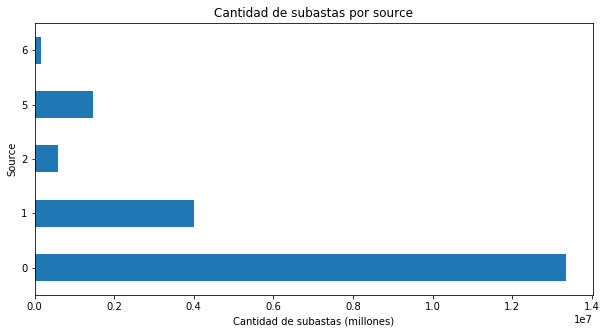
\includegraphics[width=350pt]{images/auctions/subastasporsource.png}}
		   	\caption{Cantidad de subastas para cada source}
			\label{subastassource}
		\end{figure}
	\FloatBarrier	
	

\subsection{Clicks}

\subsection{Eventos}

\subsection{Instalaciones}

\section{Análisis de archivos en conjunto}

\section{Conclusion}


\bibliographystyle{plain}
\bibliography{references}
\end{document}
